  % !TeX spellcheck = en_GB
% %%% ***************** CHAPTER INTRODUCTION ***************** %%%
\chapter{Introduction}
\label{ch:intro}
% \textcolor{red}{\textbf{The overleaf file from the Introduction is here:} \\ \url{https://www.overleaf.com/13946064tcvpbpwjzjnk}}
% \\
%%%%%%%%% INTRODUCTION %%%%%%%%%%%%%%
% \begin{itemize}
% \item General intro more specific intro (includes motivation: Why do we care?)
% \item Background / State of the art / or knowledges
% \item Open Questions
% \item short overview of your thesis
% \item Urd and the storm
% \item This is the problem and we need to do a better job in prediction
% \item Have new MEPS prediction ensemble, we are using this now to forecast this type of storms
% \item Like to see how MEPS is doing
% \item Because of NSF at Haukeliseter $\Rightarrow$ great opportunity to use to validate the mountain side
% \item Since we have snowfall obs and snowfall is important in the mountains for the safety, drinking water $\Rightarrow$ evaluate how well the model is doing for snowfall
% \end{itemize}
One of the challenges in current forecast research is the understanding and prediction of extreme weather events, such as heavy precipitation. 
Extreme winter storms with heavy precipitation can have large influence on the local infrastructure and the personal safety. Large amounts of precipitation combined with temperature changes can lead to danger in the Norwegians mountains. A better understanding of the microphysical processes in storms in crucial to better predict extreme storms. 
\\
%During Christmas 2016 an extreme storm influenced the west coast of Norway.  The storm, called 'Urd' was according to \citet{olsen_ekstremvaerrapport._2017} associated with strong winds and high precipitation amounts. 
%The average wind along the coast of Western Norway had hurricane strength (observed: \SIrange{40}{55}{\mPs}). In South and Eastern Norway west to north-west winds between \SIrange{25}{40}{\mPs} were measured.
%At the Haukeliseter measurement site, \SI{136.4}{\milli\metre} of precipitation were monitored during \SIrange{21}{27}{\dec}.
%This event was just above the limit of been called an extreme weather. 
Storms of this kind are expected to occur on average every five years \citep{olsen_ekstremvaerrapport._2017}. \\ 
The financial costs associated with 'Urd' are estimated to about 180 million Norwegian kroner.
'Urd' led to major traffic problems for cars, trains, ferries and air planes. Most mountain crossings were kept closed during Christmas 2016.  A temperature change and therefore change of precipitation from solid to liquid followed an increase in avalanche danger.
In addition, there was a power breakout of around 70.000 households and 40 emergency power stations failed during the extreme weather (\Cref{fig:news}). 
\\
This Christmas storm, might not have led to the same damages as some of the extreme weather events of recent years. But since people are affected by extreme weather (\Cref{fig:news}) it is important to predict storms, associated precipitation, wind, and temperature changes as accurately as possible. Having accurate observations, will lead to better performing models which rely on observations. \textcolor{red}{include a reference here}
%%% images from Twitter and news %%%%%%%%%%%%%%%%%%%%%%%%%%%%%%%%%%%%%
% !TeX spellcheck = en_GB
\begin{figure}[t!]
	\centering
	\begin{subfigure}[b]{0.49\textwidth}
		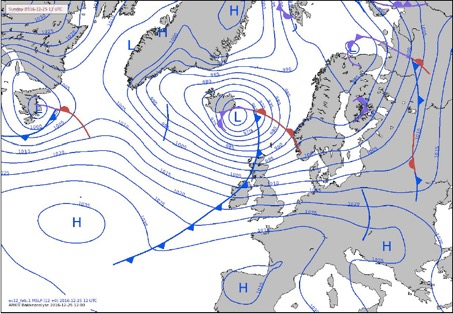
\includegraphics[width=\textwidth]{./fig_introduction/Ana_2512_12UTC.jpg}
		\caption{}\label{fig:ana_YR}
	\end{subfigure}
\hfill
	\begin{subfigure}[b]{0.49\textwidth}
		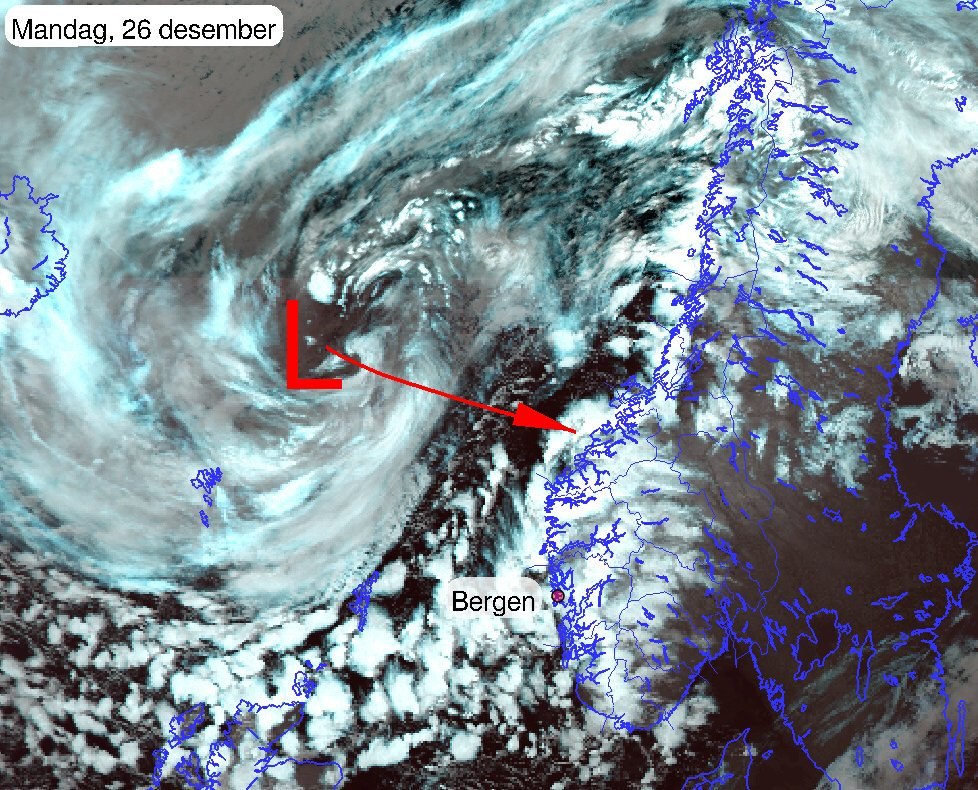
\includegraphics[trim={0cm 3.8cm 0cm 0cm},clip, width=\textwidth]{./fig_introduction/Twitter_26122016_0934AM.jpeg}
		\caption{}\label{fig:meteorologene_2612}	
	\end{subfigure}
	\begin{subfigure}[b]{0.49\textwidth}
		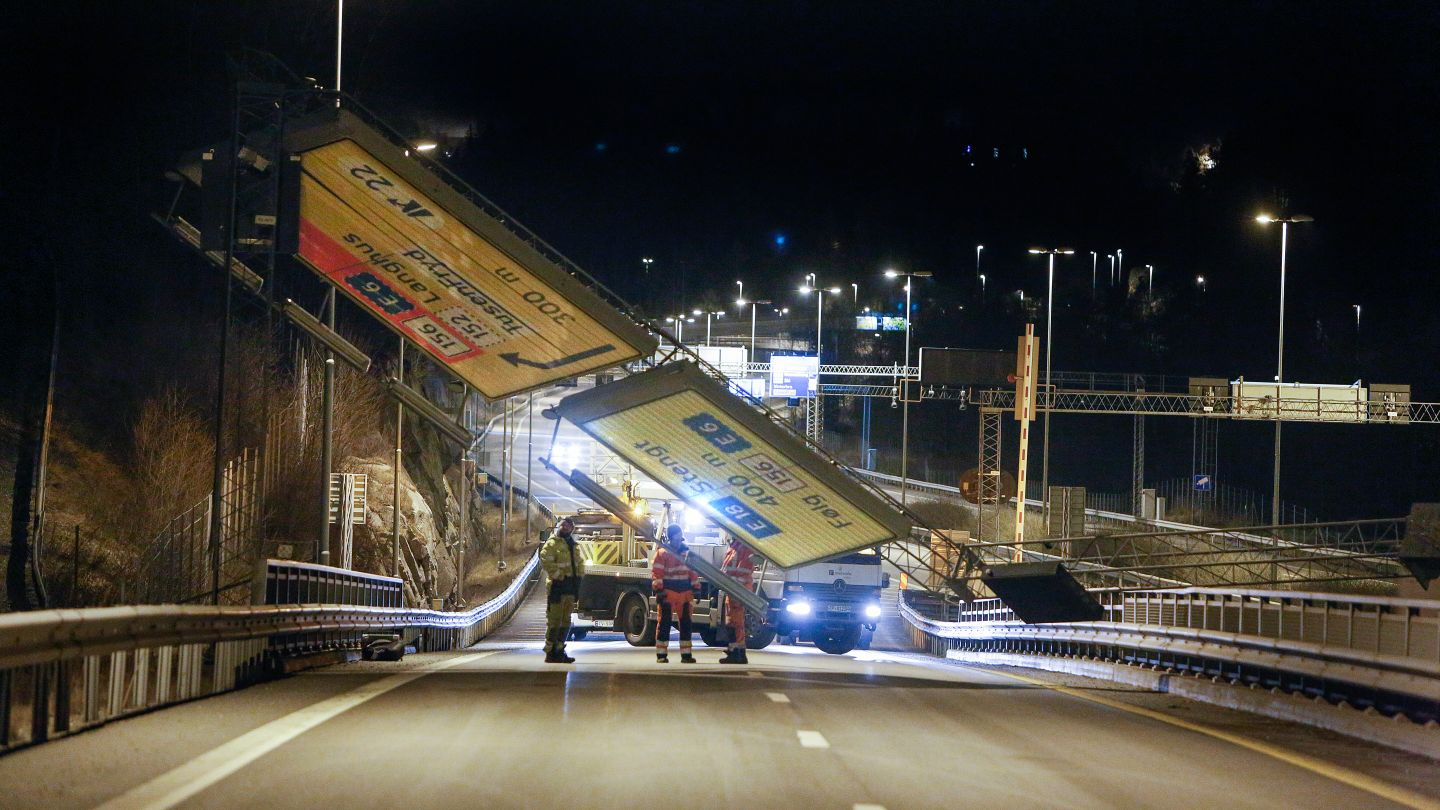
\includegraphics[width=\textwidth]{./fig_introduction/street_sign_2512.jpg}
		\caption{}\label{fig:street_sign}
	\end{subfigure}
\hfill
	\begin{subfigure}[b]{0.49\textwidth}
		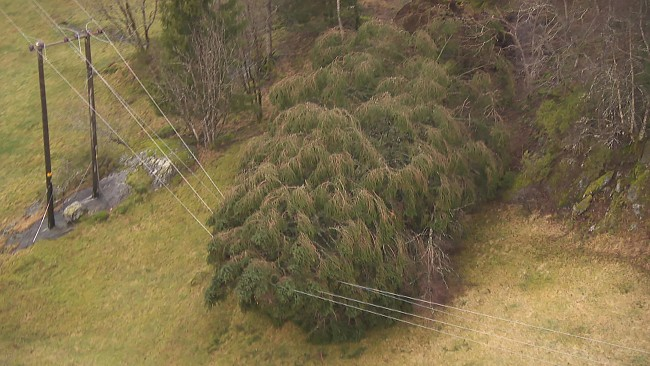
\includegraphics[width=\textwidth]{./fig_introduction/tree_nrk_2812.jpg}
		\caption{}\label{fig:tree_elec}
	\end{subfigure}
\caption{Weather situation during the extreme Christmas storm and impact on the infrastructure. In \protect\subref{fig:ana_YR}: Weather situation Sunday \SI{25}{\dec} at \SI{12}{\UTC} from the extreme weather report on Urd \citep{olsen_ekstremvaerrapport._2017}.
	\protect\subref{fig:meteorologene_2612}: Tweet from \cite{meteorologene_her_2016} on \SI{26}{\dec} at 9:34 am: Here comes \#Urd! The low pressure centre will hit M{\o}re og Romsdal, but the strongest wind comes south of Stad. \#S{\o}rNorge.
    \protect\subref{fig:street_sign} and \protect\subref{fig:tree_elec} show the consequences related to the high wind speeds during Christmas 2016.
	\protect\subref{fig:street_sign}: This traffic sign, ten meter long and four meter high was blown down during the storm, \citep{ruud_tonn_2016}.
	\protect\subref{fig:tree_elec}: Trouble maker: The extreme weather during Christmas created problems for the local infrastructure. \num{80.000} households were without electricity during the storm, \citep{farestveit_80.000_2016}.} \label{fig:news}
\end{figure}
%%%%%%%%%%%%%%%%%%%%%%%%%%%%%%%%%%%%%%%%%%%%%%%%%%%%%%%%%%%%%%%%%%%%%%%%%%
\newline
\noindent
\Cref{fig:news} shows that precipitation and strong winds can influence in certain ways the infrastructure. To predict and measure snowfall accumulation as accurately as possible is important since snowfall has impact on avalanches, freshwater release into water systems in spring, and extra economical expenses for local infrastructure as well as climatological effects. \\
% \citet{joos_influence_2012} investigated the influence of microphysical processes on potential vorticity development in warm conveyor belts (WCB). They demonstrated the complex interaction between the small-scale microphysical processes and the large-scale flow in WCB. 
% For the understanding of numerical simulations of storm developments, it is important to know vertical precipitation profiles and their position within the synoptic environment.% vorticity environment. 
It is crucial to study the vertical structure of different synoptic storms and  predict as accurately as possible.\\
% 
Since November 2016, the Meteorological Cooperation on Operational Numerical Weather Prediction (MetCoOP) Ensemble Prediction forecast (MEPS) is operational at the Meteorological Institute of Norway (Met-Norway). The ensemble prediction system uses the previous deterministic AROME-MetCoOp, a version of the Mèteo-France Applications of Research to Operations at Mesoscale and initialises in addition ten perturbed ensemble members. The use of an ensemble prediction system will give the possibility to analyse the variation of snowfall precipitation in the vertical and at the surface.
%The study by \citet{muller_arome-metcoop:_2017} shows that the AROME-MetCoOp performs well for certain meteorological phenomena, but that it has still some uncertainties by forecasting precipitation.  \\
Microphysical processes in weather models are still not well understood and therefore are mostly parametrised \citep{muller_arome-metcoop:_2017}. Furthermore, high latitude regions are not well represented in meteorological models. %Indeed, a comparison between the MEPS data fit the observations for December 2016 but uncertainties are still present for this time period. 
In this study, the newly developed ensemble prediction systems (EPS) from Met-Norway is used to analyse the extreme winter storm during Christmas 2016. It will be shown if the EPS is able to forecast the variation of an extreme winter storms such as 'Urd' and if it is able to predict large scale effects as well as local effects. 
\\
This work focuses on the measurement site Haukeliseter in Southern Norway. During winter 2016 state of the art ground measurements were installed to estimate the vertical snow water content in the atmosphere. The usage of a snowfall retrieval with ground-based measurements will give an insight to the microphysical structure of the extreme event. %This vertical and surface observations will help to verify the regional forecast model for a mountain side in Norway.
\\
Snowfall is important in the Norwegian mountains for safety and drinking water resources. The aim of this thesis is to evaluate the regional forecast model MEPS by using local observations from a mountain side in Norway. This thesis will examine research questions: How well will the model predict the surface snowfall at the measurement site? 
Does the regional model cover local affects associated with the topography around the side? Will precipitation transitions from snow to rain to snow forecasted by the regional model?
\\
The thesis is structured as following: Chapter 2 will present the synoptic analysis of the extreme storm, which will later be used to evaluate MEPS. The third chapter will give an overview of the measurement site Haukeliseter and its instrumentation. Chapter 4 and 5 covers the optimal estimation snowfall retrieval and regional model, respectively. After this will Chapter 6 present the results and discussion. The daily MEPS runs will be compared to the observed surface accumulation and the vertical retrieved snow water content. Furthermore, precipitation characteristics such as wind influence and rain segments will be discussed. The final Chapter summarises the results and findings and suggests future research which has to be done. 

%Some satellites, such as CloudSat have been equipped with radar to estimate snowfall rates and vertical profiles of precipitation. CloudSat is one of the satellites orbiting in the A-Train formation and measures the vertical structure of cloud systems \citep{stephens_cloudsat_2002}. This study is using the adapted CloudSat retrieval scheme for ground-based measurements. This will give an insight of  snowfall in the lower \SI{3}{\km} of the atmosphere. CloudSat radars are not able to observe storm structures down to \SI{3}{\km}. Using radar reflectivity from the ground can link satellite observations with ground-based observations to get a better understanding of vertical snowfall patterns.    
% \\
% Studies of \citet{kulie_utilizing_2009} showed that the Cloud Profiling Radar (CPR), mounted on the CloudSat, can be used to estimate global distributions of snowfall. They showed that different combinations of microphysical habits and fall speed can lead to the same results of reflectivity and therefore to the same amount of snowfall rate.
% Methods like optimal estimation retrieval were established to reduce the non-uniqueness. Where ground observations are used to estimate vertical profiles of precipitation.\\
% The improvement of the CloudSat retrieval is helpful to show that climate models over estimate present-day Antarctic snowfall \citep{palerme_evaluation_2017}. \citet{norin_intercomparison_2015} presented a good agreement between the ground-based snowfall measurements and satellite observations.
